\documentclass[11pt]{article}
\usepackage{geometry}
\geometry{a4paper, top=20mm, left=10mm, right=10mm, bottom=20mm}
\usepackage{graphicx}
\usepackage{amsmath,amssymb,amsthm}
\usepackage{amssymb}
\usepackage[utf8]{inputenc}
\usepackage{fancyhdr}
\usepackage{lastpage}
\usepackage{enumerate}
\usepackage{enumitem}
\usepackage{tikz}
\usetikzlibrary{shapes.geometric}
\usepackage{multicol}
\usepackage{subcaption}
\usepackage{ifthen}
%------------------------------------------ preamble
%----- fancyhdr
\fancyhead[R]{Übungsgruppe: 2 (Do 12-14)}
\fancyhead[C]{Name: Maurice Wenig}
\fancyhead[L]{Matrikelnummer: 178049}
\fancyfoot{}
\rfoot{Seite \thepage\ von \pageref{LastPage}}
\pagestyle{fancy}
%----- aufgaben
\newtheoremstyle{break}{}{5mm}{}{}{\bfseries}{}{0mm}
{\textbf{\thmname{#1}\thmnumber{ #2:} \thmnote{\textit{#3}}\newline}}
\theoremstyle{break}
\newtheorem{task}{Aufgabe}
%----- new commands
\newcommand{\Romannumeral}[1]{\MakeUppercase{\romannumeral #1}}
%----- tikz automata
\usetikzlibrary{arrows, automata, positioning}
%------------------------------------------ main
\begin{document}
%----- title
\begin{center}
\Large{Automaten und Berechenbarkeit}\\
\large{4. Übungsserie}
\end{center}
%----- tasks
\begin{task}
    \hfill\vspace{-5mm}
    \begin{enumerate}[label={(\alph*)}]
    \item $(b^* a b^* a b^* a b^* a b^* a)^*$ \\
    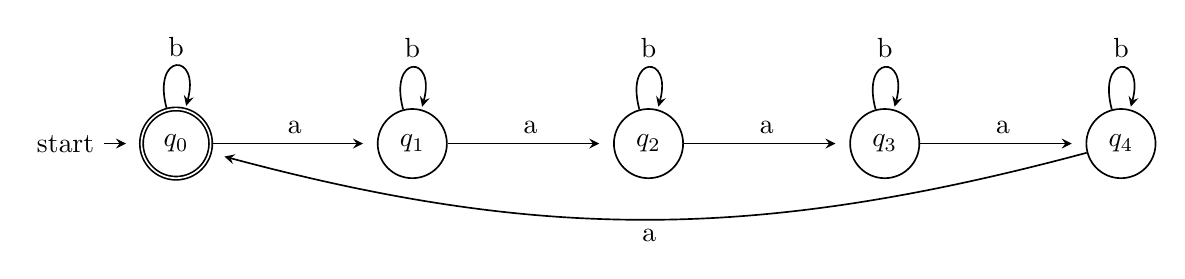
\begin{tikzpicture}[->, > = stealth, shorten > = 5 pt, node distance = 3cm, semithick]
    \node[state, initial, accepting]		(0)						{$q_0$};
    \node[state]							(1) [right of=0]			{$q_1$};
    \node[state]							(2) [right of=1] 		{$q_2$};
    \node[state]							(3) [right of=2] 		{$q_3$};
    \node[state]							(4) [right of=3] 		{$q_4$};
    \path	(0)	edge[above]					node {a}			(1);
    \path	(0)	edge[above, loop above]		node {b}			(0);
    \path	(1)	edge[above]					node {a}			(2);
    \path	(1)	edge[above, loop above]		node {b}			(1);
    \path	(2)	edge[above]					node {a}			(3);
    \path	(2)	edge[above, loop above]		node {b}			(2);
    \path	(3)	edge[above]					node {a}			(4);
    \path	(3)	edge[above, loop above]		node {b}			(3);
    \path	(4)	edge[below, bend left=15]	node {a}			(0);
    \path	(4)	edge[above, loop above]		node {b}			(4);
    \end{tikzpicture}
    
    
    \item $(b^* a a^* b b)^* \mid ((b^* a a^* b b)^* a a^*) \mid ((b^* a a^* b b)^* a a^* b)$\\
    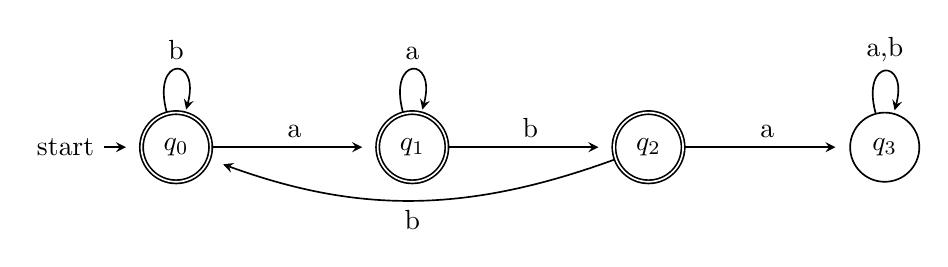
\begin{tikzpicture}[->, > = stealth, shorten > = 5 pt, node distance = 3cm, semithick]
    \node[state, initial, accepting]		(0)						{$q_0$};
    \node[state, accepting]				(1) [right of=0]			{$q_1$};
    \node[state, accepting]				(2) [right of=1] 		{$q_2$};
    \node[state]							(3) [right of=2] 		{$q_3$};
    \path	(0)	edge[above]					node {a}			(1);
    \path	(0)	edge[above, loop above]		node {b}			(0);
    \path	(1)	edge[above]					node {b}			(2);
    \path	(1)	edge[above, loop above]		node {a}			(1);
    \path	(2)	edge[above]					node {a}			(3);
    \path	(2)	edge[below, bend left=20]	node {b}			(0);
    \path	(3)	edge[above, loop above]		node {a,b}		(3);
    \end{tikzpicture}
    
    
    \item $a^*\mid (a^* b a)^*\mid ((a^* b a)^* b)\mid ((a^* b a)^* b b^*)\mid ((a^* b a)^* b (b^* a b)^*) \mid ((a^* b a)^* b (b^* a b)^* a)$\\
    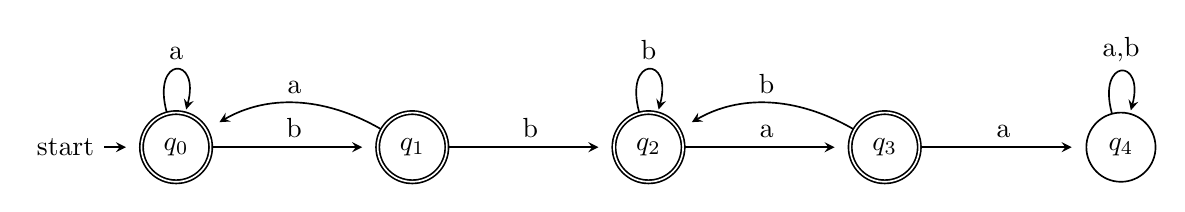
\begin{tikzpicture}[->, > = stealth, shorten > = 5 pt, node distance = 3cm, semithick]
    \node[state, initial, accepting]		(0)						{$q_0$};
    \node[state, accepting]				(1) [right of=0]			{$q_1$};
    \node[state, accepting]				(2) [right of=1] 		{$q_2$};
    \node[state, accepting]				(3) [right of=2] 		{$q_3$};
    \node[state]							(4) [right of=3] 		{$q_4$};
    \path	(0)	edge[above]					node {b}			(1);
    \path	(0)	edge[above, loop above]		node {a}			(0);
    \path	(1)	edge[above, bend right]		node {a}			(0);
    \path	(1)	edge[above]					node {b}			(2);
    \path	(2)	edge[above]					node {a}			(3);
    \path	(2)	edge[above, loop above]		node {b}			(2);
    \path	(3)	edge[above]					node {a}			(4);
    \path	(3)	edge[above, bend right]		node {b}			(2);
    \path	(4)	edge[above, loop above]		node {a,b}			(4);
    \end{tikzpicture}
    \end{enumerate}
\end{task}

\begin{task}
    \hfill\vspace{-5mm}
    \begin{enumerate}[label={\arabic*.}]
        \item $N_{Sp} = (Q\cup \{q_0'\}, \Sigma, \delta', q_0', F'), F' = \{ q_0 \}, \delta'(q, x) := 
        \begin{cases}
            F & \text{falls } q=q_0', x=\lambda \\
            p & \text{falls } \delta(p, x) = q, q\in Q, p\in Q, x\in \Sigma_\lambda\\
            \emptyset & \text{sonst}
        \end{cases}\\
        \text{wobei } Q\cap \{q_0'\} =  \emptyset
        $
        \item \hfill\vspace{-5mm}
        \begin{align*}
            Sp(L(N)) &= \{ Sp(w)\mid w\in L(N) \} \\
            &= \{ Sp(w)\mid \delta^*(q_0, w) \in F \}\\
            &= \{ Sp(w) \mid \delta'^*(F, Sp(w)) = q_0 \}\\
            &= \{ w \mid \delta'^*(q_o', w) \in F' \}\\
            &= \underline{\underline{L(N_{Sp})}}
        \end{align*}
    \end{enumerate}
\end{task}

\begin{task}
    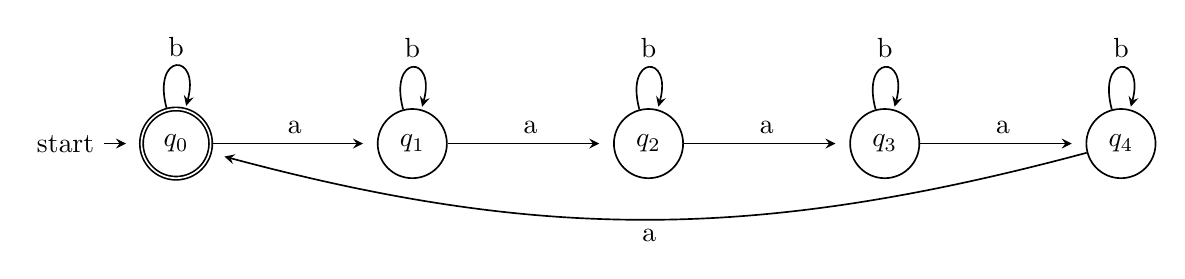
\begin{tikzpicture}[->, > = stealth, shorten > = 5 pt, node distance = 3cm, semithick]
        \node[state, initial, accepting]		(0)						{$q_0$};
        \node[state]							(1) [right of=0]			{$q_1$};
        \node[state]							(2) [right of=1] 		{$q_2$};
        \node[state]							(3) [right of=2] 		{$q_3$};
        \node[state]							(4) [right of=3] 		{$q_4$};
        \path	(0)	edge[above]					node {a}			(1);
        \path	(0)	edge[above, loop above]		node {b}			(0);
        \path	(1)	edge[above]					node {a}			(2);
        \path	(1)	edge[above, loop above]		node {b}			(1);
        \path	(2)	edge[above]					node {a}			(3);
        \path	(2)	edge[above, loop above]		node {b}			(2);
        \path	(3)	edge[above]					node {a}			(4);
        \path	(3)	edge[above, loop above]		node {b}			(3);
        \path	(4)	edge[below, bend left=15]	node {a}			(0);
        \path	(4)	edge[above, loop above]		node {b}			(4);
        \end{tikzpicture}
\end{task}
\end{document}
